\chapter{Experiments}


\section{Introduction}

As we have seen in the previous section, all results of a simulation are stored into several \texttt{.csv} files.

\begin{itemize}
    \item \texttt{states.csv} contains, for each State, its id, population size, VAT rate, levy rate, tariff rate, wealth tax rate, allowance type, unemployment rate, black economy share, GDP, the money it has, the total money of its population (agents), the number of transactions performed by its agents, and the id's of the other States to which it is connected.

    \item \texttt{agents.csv} contains, for each Agent, its id, the id of its State, its initial money (the money with each it started the simulation), its current money, its talent, whether it is a producer or not (thus whether it is employed or unemployed) and the number of purchases it has made.
    
    \item \texttt{products.csv} contains, for each Agent, the id of the Agent producing it, its type, the production price (always set to 0), the selling price, the stock of this product, and the number of sales. Therefore, each agent has one Product and we can merge this file with the agents file.
    
    \item \texttt{ticks.csv} keeps track of different values during the simulation. The following metrics are saved every 100 ticks: the number of ticks that have passed so far, the number of transactions that have happened in the World so far, the total money of all the States, the total money of all the Agents, and the total GDP of all States.
\end{itemize}

Based on these files, we can do various experiments by adjusting the parameters and see the effects on some key metrics. For this, the language Python3 has been chosen as it contains many libraries to analyze and plot such data: pandas, numpy or matplotlib. Rapidness is not the key factor here as the simulation has already stored its results in the \texttt{.csv} files.

The default configuration file that we use is the following. Experiment after experiment, we will modify one or several parameter and see its/their influence. 

\begin{lstlisting}[language=json,firstnumber=1]
{
    "World": {
        "PRODUCT_CHOICE": "CHEAPEST",
        "NB_STATES": 200,
        "NB_AGENTS": 30000,
        "NB_TICKS": 4000,
        "NB_TICKS_SAVE_CSV": 100
    },
    "Connections": {
        "CLUSTER_SIZE": 0,
        "PROB_CONNECTION": 0.0
    },
    "State": {
        "Tax": {
            "MIN_VAT": 0.2,
            "MAX_VAT": 0.2,
            "MIN_LEVY": 0.1,
            "MAX_LEVY": 0.1,
            "MIN_TARIFF": 0.3,
            "MAX_TARIFF": 0.3,
            "VAL_WEALTH_TAX_TOP": 0.1,
            "MIN_WEALTH_TAX_VALUE": 0.2,
            "MAX_WEALTH_TAX_VALUE": 0.2,
            "NB_TICKS_COLLECT_TAXES": 100
        },
        "Allowance": {
            "NB_TICKS_DISTRIBUTE_ALLOWANCES": 100
        },
        "Others": {
            "MIN_UNEMPLOYMENT": 0.05,
            "MAX_UNEMPLOYMENT": 0.05,
            "MIN_BLACK": 0.15,
            "MAX_BLACK": 0.15
        }
    },
    "Agent": {
        "MIN_INIT_MONEY": 1000.0,
        "MAX_INIT_MONEY": 1000.0,
        "RATIO_BUY": 0.5,
        "RATIO_PRODUCE": 0.5
    },
    "Product": {
        "NB_DIFF_PRODUCTS": 50,
        "MIN_PRICE": 0.0,
        "MAX_PRICE": 300.0,
        "MAX_STOCK": 2000
    }
}
\end{lstlisting}

Whenever points are scattered on a plot, we will also plot a line which interpolates, with a degree 2, these points to better highlight the trend. Also, in the bar charts, an average is computed in order to give a global overview. We also have to pay attention that most plots have two $y$ axis (red is for the left hand-side, blue for the right hand-side). There are over 40 plots in the folder \texttt{./report/img/exp/}, we will only focus on the most interesting ones.

For each experiment, we will compare it with the state-of-the-art presented earlier, and try to answers the many research questions introduced in the section~\ref{section:motivation_objectives}.


\section{State experiments}

We will start our experiments with all the parameters related to the State. We should note that to be able to compare fairly different States, the metrics of the State (for instance the total money of its Agents or the GDP) is divided by its population size. 

    \subsection{Experiment 1: No taxes}
    In this first experiment, we will try to see the effects on having no taxes (thus all tax values are set to 0). In the following plots, we will plot the State with regular taxes (as defined earlier) on the left hand-side, and the State with no taxes on the right hand-size. 

        \subsubsection{State GDP and number of transactions}

        We can see on the following plots that a State with no taxes (thus VAT of 0, but the other taxes are also set to 0) will generally have a smaller GDP and the number of transactions is also decreased compared to a State with taxes (left plot where the VAT is 0.2 for instance). 
        
        At first this might seem rather odd since we expect products to be cheaper, therefore more transactions should be happening (hence the GDP would be boosted too). However, if we think more about it, this seems rather logical because a State with no tax will not be able to distribute allowances, and thus some agents will concentrate all the money at the expense of other agents who will not be able to buy products anymore after some time, eventually diminishing both the GDP and the number of transactions.

        \begin{figure}[H]
            \minipage{0.5\textwidth}
                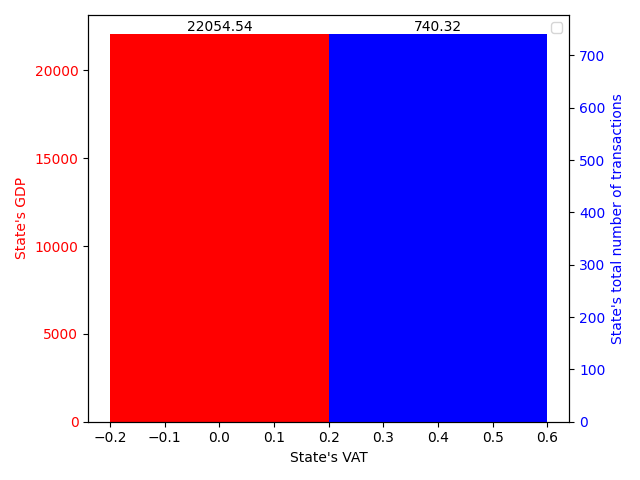
\includegraphics[width=\linewidth]{img/exp/1_1_1.png}
                \caption{Normal taxes (e.g. VAT of 0.2)}
            \endminipage\hfill
            \minipage{0.5\textwidth}
                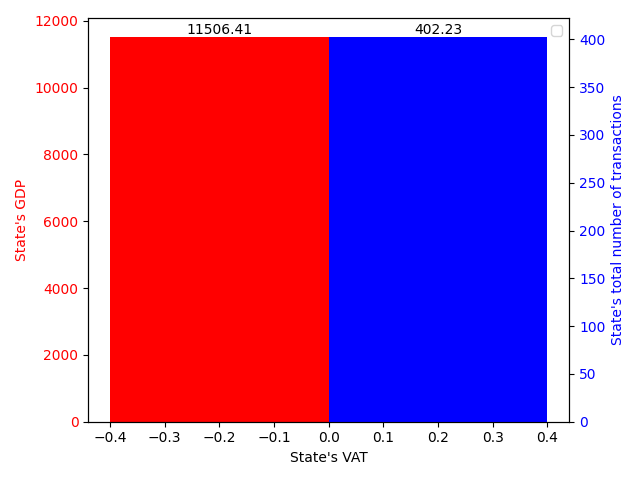
\includegraphics[width=\linewidth]{img/exp/1_2_1.png}
                \caption{No taxes (e.g. VAT of 0)}
            \endminipage\hfill
        \end{figure}

        \subsubsection{Gini coefficient} 
        
        Another interesting metric is the measure of inequalities, i.e. the Gini coefficient, the smaller it is, the more equal a society is. We can, naturally, see a tremendous difference between the two plots. Indeed, if the State has no taxes, it cannot collect nor distribute money. Therefore, the Gini coefficient skyrockets from $0.36$ to $0.91$.

        \begin{figure}[H]
            \minipage{0.5\textwidth}
                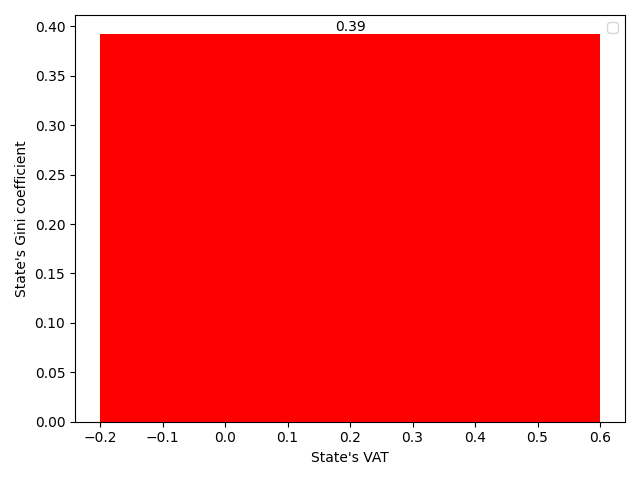
\includegraphics[width=\linewidth]{img/exp/1_1_3.png}
                \caption{Normal taxes (e.g. VAT of 0.2)}
            \endminipage\hfill
            \minipage{0.5\textwidth}
                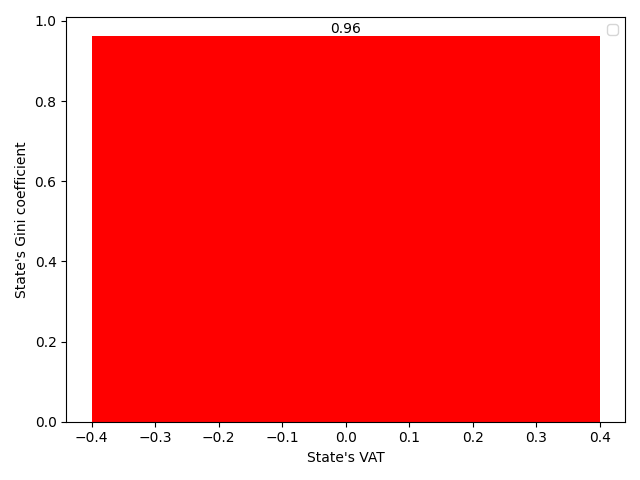
\includegraphics[width=\linewidth]{img/exp/1_2_3.png}
                \caption{No taxes (e.g. VAT of 0)}
            \endminipage\hfill
        \end{figure}

        This experiment shows the importance of having taxes (in the broadest sense of the term) on several metrics in order for our society to advance and be more fair.

    \subsection{Experiment 2: VAT}
    We will now, for each of the four taxes that were presented, analyze their influence. First: the VAT. For this, we will generate many States with random values for the VAT (ranging from 0 to 1) and see if we can see any pattern emerging regarding some metrics.

        \subsubsection{State GDP and number of transactions}

        \begin{wrapfigure}{l}{0.5\linewidth}
            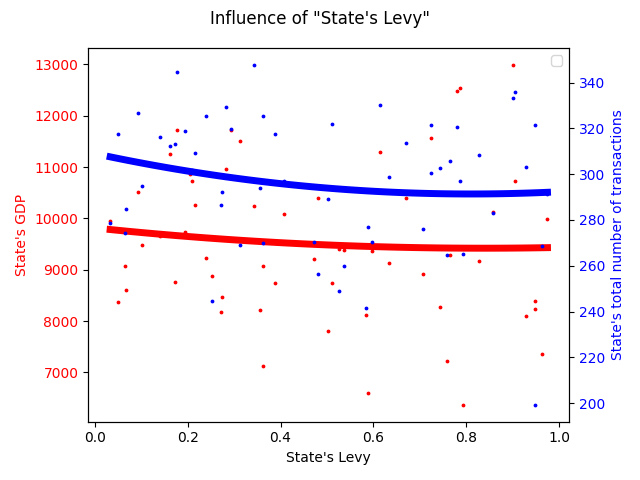
\includegraphics[width=\linewidth]{img/exp/2_1.png}
        \end{wrapfigure} 
        {Although the trend is not totally linear, we can still see a rather interesting correlation between the VAT of a State and its GDP and the number of transactions happening. As we can see on the plot, being in either of the two extremes (VAT close to 0 or to 1) is rather detrimental. Indeed, as we have seen in the previous experiment, having a very low VAT is bad for our these two metrics. However, having it too high is also problematic (close to 1 would mean that a product costing 100 will now cost 200) because products are now much more expensive, therefore agents will make fewer purchases and the GDP will be lowered too. 
        \par

        \subsubsection{Gini coefficient}

        \begin{wrapfigure}{r}{0.5\linewidth}
            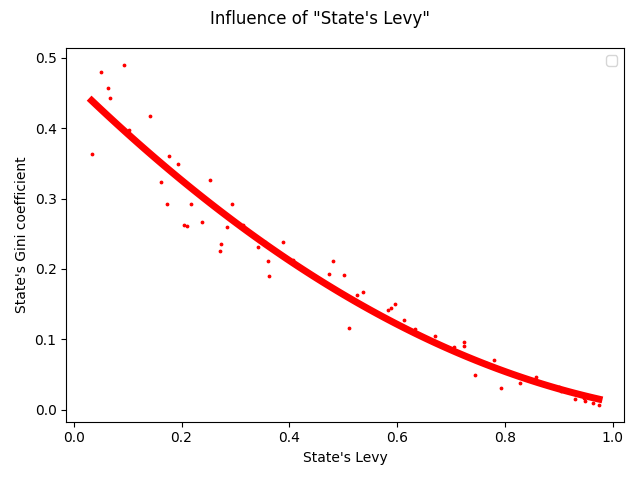
\includegraphics[width=\linewidth]{img/exp/2_3.png}
        \end{wrapfigure} 
        {Naturally, as we had seen before, the lower the VAT is, the more inequalities we will have since the State has less money to redistribute fairly. However, we can see that here, with a VAT of 0, the Gini coefficient is around 0.45 whereas it was at 0.91 before. This is because in this case, the other taxes are still present as shown in the default configuration allowing the State to distribute allowances and diminishing inequalities. Hence why the higher the VAT is, the less inequalities we have since the Gini coefficient tends to go to zero.
        \par

    \subsection{Experiment 3: Tariff}
    As for the VAT, we will now analyze the influence of the tariff tax by generating many States with random values (ranging from 0 to 1) and see if we can see any pattern emerging regarding some metrics. 

        %TODO


    \subsection{Experiment 4: Levy}
    We will now analyze the influence of the levy tax by generating many States with random values (ranging from 0 to 1) and see if we can see any pattern emerging regarding some metrics. 

        %TODO


    \subsection{Experiment 5: Wealth tax}
    We will now analyze the influence of the last tax: the wealth tax with the same methodologies as the previous taxes and see if we can see any pattern emerging regarding some metrics. 

        %TODO


    \subsection{Experiment 6: Unemployment}
    After analyzing the different taxes, we will now focus on another parameter which cannot directly be controlled by the State. As usual, we will create many States with different unemployment rates and see how our metrics change.

            
        \subsubsection{State GDP and number of transactions}

        \begin{wrapfigure}{l}{0.5\linewidth}
            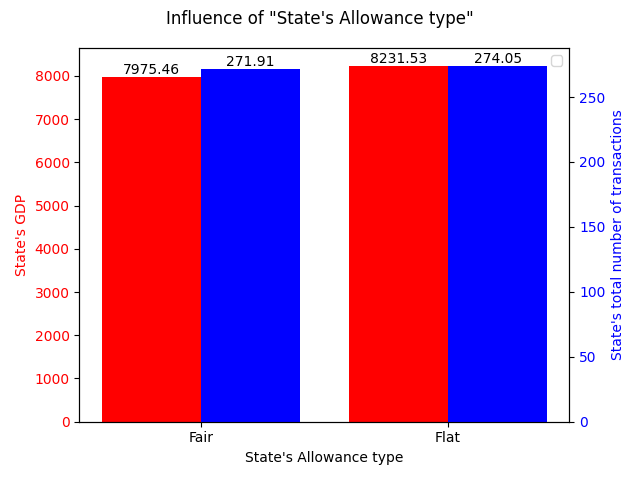
\includegraphics[width=\linewidth]{img/exp/6_1.png}
        \end{wrapfigure} 
        {As one could have expected, we have a rather clear linear correlation. Indeed, the higher the unemployment rate is, the less number of transactions we have and the lower the GDP is. Actually, it is a vicious cycle because the less producers we have, the less products are available on the market, thus less transactions. By having less transactions, we collect less taxes, and therefore do not distribute as much, this means that some agents will never be able to buy another product. 
        \par

        \subsubsection{Gini coefficient}

        \begin{wrapfigure}{r}{0.5\linewidth}
            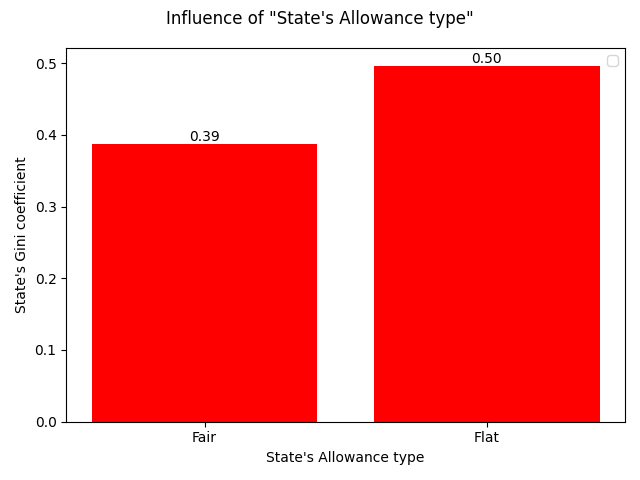
\includegraphics[width=\linewidth]{img/exp/6_3.png}
        \end{wrapfigure} 
        {The plot on the side is a bit tricky but more interesting to analyze. If we only look at the scattered points, we see that there is a linear correlation from the rate 0.0 until 0.8: the more non-producing agents we have, the bigger the Gini coefficient is. This is logical because producing agents will still be able to sell their products and make some money thus accumulating more wealth compared to others, increasing the inequalities.

        However, after the 0.8 rate on the $x$ axis, we can see a significant drop, and the previous statement does not hold true anymore: the Gini coefficient gets very close to zero, i.e. perfect equality. Actually, it also makes sense because if almost everybody is unemployed, then no one can afford to buy any product, thus we have almost no transactions happening and no money flowing between agents, and no agent can therefore become richer than others.
        \par


    \subsection{Experiment 7: Black economy}
    The second parameter which cannot directly be controlled by the State is the black economy. As usual, we will create many States with different share of black economy happening and see how our metrics change.

            
        \subsubsection{State GDP and number of transactions}

        \begin{wrapfigure}{l}{0.5\linewidth}
            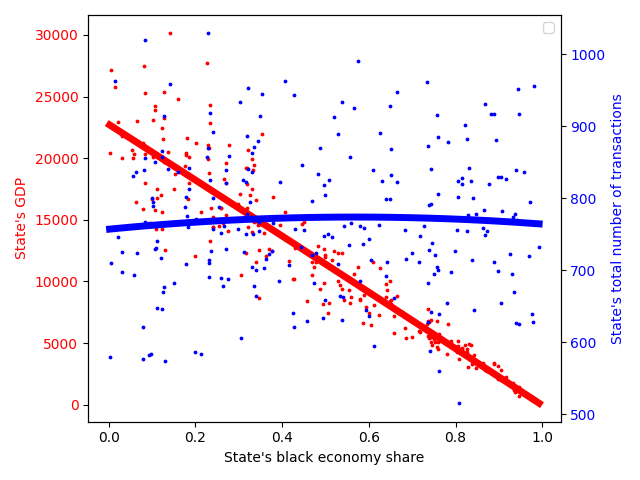
\includegraphics[width=\linewidth]{img/exp/7_1.png}
        \end{wrapfigure} 
        {We see almost no correlation. This is due to the fact that black transactions are still counted as transactions. As for the GDP, however \\ \\ \\ \\ \\%TODO 
        \par

        \subsubsection{Gini coefficient}

        \begin{wrapfigure}{r}{0.5\linewidth}
            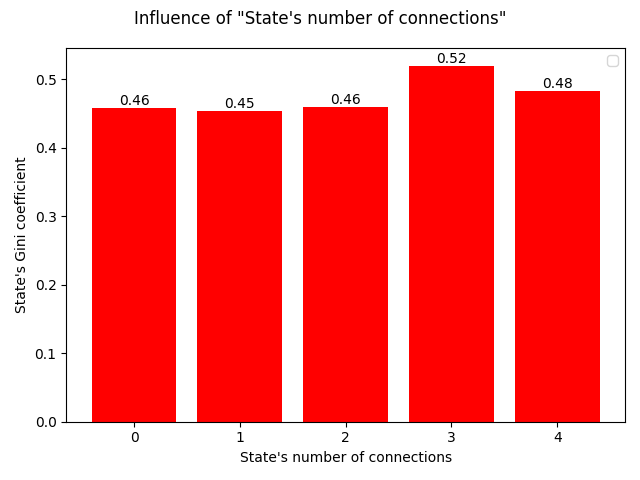
\includegraphics[width=\linewidth]{img/exp/7_3.png}
        \end{wrapfigure} 
        {As the black economy share increases, the inequalities augment as well. This is simply due to the fact that the State will have less money to redistribute when giving allowances, therefore inequalities will subsist even after the small amount of money collected as been redistributed. \\ \\
        \par
    


    \subsection{Experiment 8: Allowances}
    
    

    
%\section{Agent experiments}
    
%\section{Product experiments}